\chapter{Dodatek A}
\section{Dodatkowe predykcje}
\label{Dodatek_A}

\todo[inline]{Na pewno sugerowałbym, aby mimo tego, że to dodatek, to do każdego rysunku dodać opis w tekście z przypisem...}

\subsection*{Predykcje modeli bazowych}

\begin{figure}[h]
    \centering
    \subfloat[][YOLOv8n]{
    
\includegraphics[width = 0.3\textwidth]{Pics/Predictions/Sacred/YOLO8/Baseline/sacred_1_R001_C001.jpg}
    \label{fig:baseline_yolov8n_1}}
    \quad
    \subfloat[][YOLOv26n]{
    
\includegraphics[width = 0.3\textwidth]{Pics/Predictions/Sacred/YOLO26/Baseline/sacred_1_R001_C001.jpg}
    \label{fig:baseline_yolov26n_1}}
    \quad
    \subfloat[][RT-DETR-L]{
    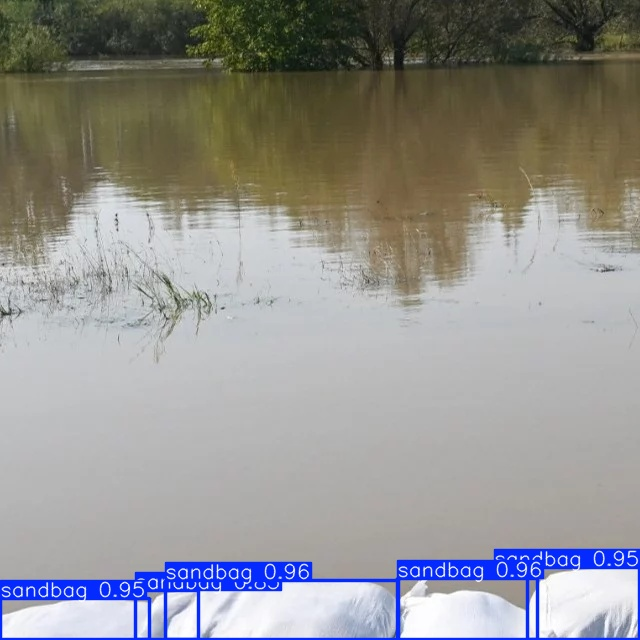
\includegraphics[width = 0.3\textwidth]{Pics/Predictions/Sacred/RT-DETR-L/Baseline/sacred_1_R001_C001.jpg}
    \label{fig:baseline_rtdetr_1}}
    \caption{Porównanie predykcji modeli bazowych dla obrazu spoza zbioru treningowego.}
    \label{fig:baseline_comparison_1}
\end{figure}

\begin{figure}[h]
    \centering
    \subfloat[][YOLOv8n]{
    
\includegraphics[width = 0.3\textwidth]{Pics/Predictions/Sacred/YOLO8/Baseline/sacred_3.jpg}
    \label{fig:baseline_yolov8n_2}}
    \quad
    \subfloat[][YOLOv26n]{
    
\includegraphics[width = 0.3\textwidth]{Pics/Predictions/Sacred/YOLO26/Baseline/sacred_3.jpg}
    \label{fig:baseline_yolov26n_2}}
    \quad
    \subfloat[][RT-DETR-L]{
    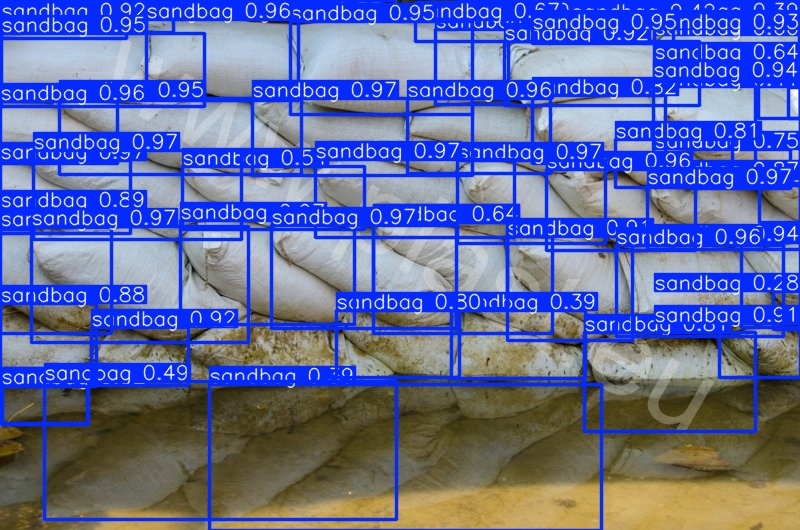
\includegraphics[width = 0.3\textwidth]{Pics/Predictions/Sacred/RT-DETR-L/Baseline/sacred_3.jpg}
    \label{fig:baseline_rtdetr_2}}
    \caption{Porównanie predykcji modeli bazowych dla obrazu spoza zbioru treningowego.}
    \label{fig:baseline_comparison_2}
\end{figure}

\subsection*{Predykcje modeli z metody A}

\begin{figure}[h]
    \centering
    \subfloat[][YOLOv8n]{
    
\includegraphics[width = 0.3\textwidth]{Pics/Predictions/Sacred/YOLO8/Pseudo/sacred_1_R001_C001.jpg}
    \label{fig:pseudo_yolov8n_1}}
    \quad
    \subfloat[][YOLOv26n]{
    
\includegraphics[width = 0.3\textwidth]{Pics/Predictions/Sacred/YOLO26/Pseudo/sacred_1_R001_C001.jpg}
    \label{fig:pseudo_yolov26n_1}}
    \quad
    \subfloat[][RT-DETR-L]{
    
\includegraphics[width = 0.3\textwidth]{Pics/Predictions/Sacred/RT-DETR-L/Pseudo/sacred_1_R001_C001.jpg}
    \label{fig:pseudo_rtdetr_1}}
    \caption{Porównanie predykcji modeli po zastosowaniu pseudo-etykietowania dla obrazu spoza zbioru treningowego.}
    \label{fig:pseudo_comparison_1}
\end{figure}

\begin{figure}[h]
    \centering
    \subfloat[][YOLOv8n]{
    
\includegraphics[width = 0.3\textwidth]{Pics/Predictions/Sacred/YOLO8/Pseudo/sacred_3.jpg}
    \label{fig:pseudo_yolov8n_2}}
    \quad
    \subfloat[][YOLOv26n]{
    
\includegraphics[width = 0.3\textwidth]{Pics/Predictions/Sacred/YOLO26/Pseudo/sacred_3.jpg}
    \label{fig:pseudo_yolov26n_2}}
    \quad
    \subfloat[][RT-DETR-L]{
    
\includegraphics[width = 0.3\textwidth]{Pics/Predictions/Sacred/RT-DETR-L/Pseudo/sacred_3.jpg}
    \label{fig:pseudo_rtdetr_2}}
    \caption{Porównanie predykcji modeli po zastosowaniu pseudo-etykietowania dla obrazu spoza zbioru treningowego.}
    \label{fig:pseudo_comparison_2}
\end{figure}

\subsection*{Predykcje modeli z metody B}

\begin{figure}[h]
    \centering
    \subfloat[][YOLOv8n]{
    
\includegraphics[width = 0.3\textwidth]{Pics/Predictions/Sacred/YOLO8/Generative/sacred_1_R001_C003.jpg}
    \label{fig:generative_yolov8n_1}}
    \quad
    \subfloat[][YOLOv26n]{
    
\includegraphics[width = 0.3\textwidth]{Pics/Predictions/Sacred/YOLO26/Generative/sacred_1_R001_C003.jpg}
    \label{fig:generative_yolov26n_1}}
    \quad
    \subfloat[][RT-DETR-L]{
    
\includegraphics[width = 0.3\textwidth]{Pics/Predictions/Sacred/RT-DETR-L/Generative/sacred_1_R001_C003.jpg}
    \label{fig:generative_rtdetr_1}}
    \caption{Porównanie predykcji modeli po zastosowaniu Metody B dla obrazu spoza zbioru treningowego.}
    \label{fig:generative_comparison_1}
\end{figure}

\begin{figure}[h]
    \centering
    \subfloat[][YOLOv8n]{
    
\includegraphics[width = 0.3\textwidth]{Pics/Predictions/Sacred/YOLO8/Generative/sacred_1_R001_C001.jpg}
    \label{fig:generative_yolov8n_2}}
    \quad
    \subfloat[][YOLOv26n]{
    
\includegraphics[width = 0.3\textwidth]{Pics/Predictions/Sacred/YOLO26/Generative/sacred_1_R001_C001.jpg}
    \label{fig:generative_yolov26n_2}}
    \quad
    \subfloat[][RT-DETR-L]{
    
\includegraphics[width = 0.3\textwidth]{Pics/Predictions/Sacred/RT-DETR-L/Generative/sacred_1_R001_C001.jpg}
    \label{fig:generative_rtdetr_2}}
    \caption{Porównanie predykcji modeli po zastosowaniu Metody B dla obrazu spoza zbioru treningowego.}
    \label{fig:generative_comparison_2}
\end{figure}

\begin{figure}[h]
    \centering
    \subfloat[][YOLOv8n]{
    
\includegraphics[width = 0.3\textwidth]{Pics/Predictions/Sacred/YOLO8/Generative/sacred_3.jpg}
    \label{fig:generative_yolov8n_3}}
    \quad
    \subfloat[][YOLOv26n]{
    
\includegraphics[width = 0.3\textwidth]{Pics/Predictions/Sacred/YOLO26/Generative/sacred_3.jpg}
    \label{fig:generative_yolov26n_3}}
    \quad
    \subfloat[][RT-DETR-L]{
    
\includegraphics[width = 0.3\textwidth]{Pics/Predictions/Sacred/RT-DETR-L/Generative/sacred_3.jpg}
    \label{fig:generative_rtdetr_3}}
    \caption{Porównanie predykcji modeli po zastosowaniu Metody B dla obrazu spoza zbioru treningowego.}
    \label{fig:generative_comparison_3}
\end{figure}